% -*- Mode:TeX -*-
% LaTeX template for CinC papers                   v 1.1a 22 August 2010
%
% To use this template successfully, you must have downloaded and unpacked:
%       http://www.cinc.org/authors_kit/papers/latex.tar.gz
% or the same package in zip format:
%       http://www.cinc.org/authors_kit/papers/latex.zip
% See the README included in this package for instructions.
%
% If you have questions, comments or suggestions about this file, please
% send me a note!  George Moody (george@mit.edu)
%
\documentclass[twocolumn]{cinc}
\usepackage{graphicx}
\usepackage{amsmath}
\usepackage{amsfonts}

\begin{document}
\bibliographystyle{cinc}

\title{Dynamic Time Warping with Gradient Boosting Tree Ensemble for \\
12-Lead Electrocardiogram Multilabel Classification}

\author {Alexander W Wong$^{1}$, Weijie Sun$^{2}$, Sunil V Kalmady$^{2}$, Padma Kaul$^{2}$, Abram Hindle$^{1}$\\
\ \\
 $^1$ University of Alberta, Edmonton, Canada \\
$^2$ Canadian VIGOUR Center, Edmonton, Canada }

\maketitle

\begin{abstract}

Standard 12-lead electrocardiograms (ECGs) are commonly used to detect cardiac irregularities such as atrial fibrillation, blocks and irregular complexes.
For the Physionet/CinC 2020 Challenge, we built an algorithm using gradient boosted tree ensembles fitted on morphology and signal processing features.

We used the \emph{ecgpuwave} implementation of the Pan Tompkins method to detect the P-wave, QRS complex, and T-wave.
We selected templates that exhibited maximum similarity with the rest of the ECG records in the same class using minimum distance criteria to isolate candidate templates for each cardiac abnormality.
We leveraged these templates using Dynamic Time Warping (DTW), an algorithm used for measuring similarity between temporal sequences of varying speeds.
From the annotated signals we derived additional features related to their durations, amplitudes, and intervals.

We concatenated the features for all 12 leads to fit an ensemble of gradient boosting trees and predicted probabilities of ECG instances belonging to each class.
We evaluated using a 5-fold cross validation split of the provided dataset.
TODO: new scoring metric

\end{abstract}

\section{Introduction}

Cardiovascular diseases are a non-communicable leading cause of death, responsible for an estimated 17.8 million fatalities world wide in 2017~\cite{roth_global_2018}.
The electrocardiogram (ECG) is the most effective tool and current best practice strategy for detecting cardiac diseases, outperforming screening history and physical examinations in accuracy and sensitivity~\cite{harmon_effectiveness_2015}.
However, ECG interpretation is a complex and highly skilled task undertaken by multiple health care professionals ranging from physicians, nurses, paramedics, and technicians.
Multiple studies have been conducted highlighting disagreements between non-cardiologists and cardiologist reference ECG interpretations, with up to a 33\% interpretation error rate~\cite{mele_improving_2008}.
Despite active research in computerized interpretations of ECGs, trained human over-reading and confirmation is required and emphasized in published reports~\cite{schlapfer_computer-interpreted_2017}.

This work classifies standard 12-lead ECGs to their clinical diagnosis as part of the \emph{PhysioNet/Computing in Cardiology Challenge}~\cite{physionet_challenge_2020}.
We developed a multi-label classification algorithm using natural language and signal processing inspired features and a gradient boosting tree ensemble.

\subsection{Dataset \& Scoring Criteria}

The official phase dataset contained a total of 43,101 ECG records.
After dropping 6 records that had less half or more of their leads zero'd out, the remaining 43,095 records were used for further analysis.
Each record was labeled with one or more SNOMED CT codes, with 123 different labels observed in the provided data.

\begin{table}[htbp]
  \caption{\label{tab:dataset_labeldx} Top 7 labels within the provided dataset.}
  \vspace{4 mm}
  \centerline{\begin{tabular}{lrr} \hline
    Label                        & Percent & Count \\ \hline
    sinus rhythm                 &  48.4\% & 20846 \\
    left axis deviation          &  14.1\% &  6086 \\
    myocardial infarction        &  14.0\% &  6019 \\
    t wave abnormal              &  10.8\% &  4673 \\
    left ventricular hypertrophy &   8.7\% &  3760 \\
    nonspecific st t abnormality &   8.3\% &  3557 \\
    atrial fibrillation          &   8.1\% &  3473 \\ \hline
  \end{tabular}}
\end{table}

Table~\ref{tab:dataset_labeldx} highlights the label imbalance, with over 87\% of the dataset diagnosed as one of the four most common labels.
Approximately 55\% of the dataset is classified with more than one label, as shown in Table~\ref{tab:dataset_multidx}.

\begin{table}[htbp]
  \caption{\label{tab:dataset_multidx} Dataset multi-label records proportion.}
  \vspace{4 mm}
  \centerline{\begin{tabular}{lrr} \hline
    Labels Per Record & Percent & Count \\ \hline
        1 & 45.2\% & 19461 \\
        2 & 21.8\% & 9378  \\
        3 & 14.9\% & 6426 \\
        4 &  9.9\% & 4280 \\
        5 &  4.9\% & 2113 \\
        6 &  2.2\% & 935 \\
        7 &  0.8\% & 359 \\
     $>7$ &  0.3\% & 143 \\\hline
  \end{tabular}}
\end{table}

TODO: Scoring criteria, when released

\section{Methodology}

Our approach is inspired by existing methods which use feature engineering and shallow learning classifiers~\cite{tziakouri_identification_2017, goodwin_classification_2017}.

\begin{equation}
  \label{eq:dtw}
  \text{DTW}(X, Y) = \min_W(\sum_{h=1}^{P}(w_k))
\end{equation}

Dynamic Time Warping (DTW) allows us to perform template matching of variable length time-series using a non-linear transformation.
Given two time-series $X := (x_1, x_2, \ldots, x_N)$ and $Y := (y_1, y_2, \ldots, y_M)$, where $N, M \in \mathbb{N}$, an $N \times M$ matrix is constructed containing the distance of values $d(x_i, y_j)$.
A warping path $W := (w_1, w_2, \ldots, w_k)$ aligns the elements of $X$ and $Y$ such that the distance between them is minimized.
DTW is defined in equation~\ref{eq:dtw} as the minimization over potential warping paths based on the cumulative distance for each path~\cite{berndt_using_1994}.

\begin{figure}[h]
  \centering
  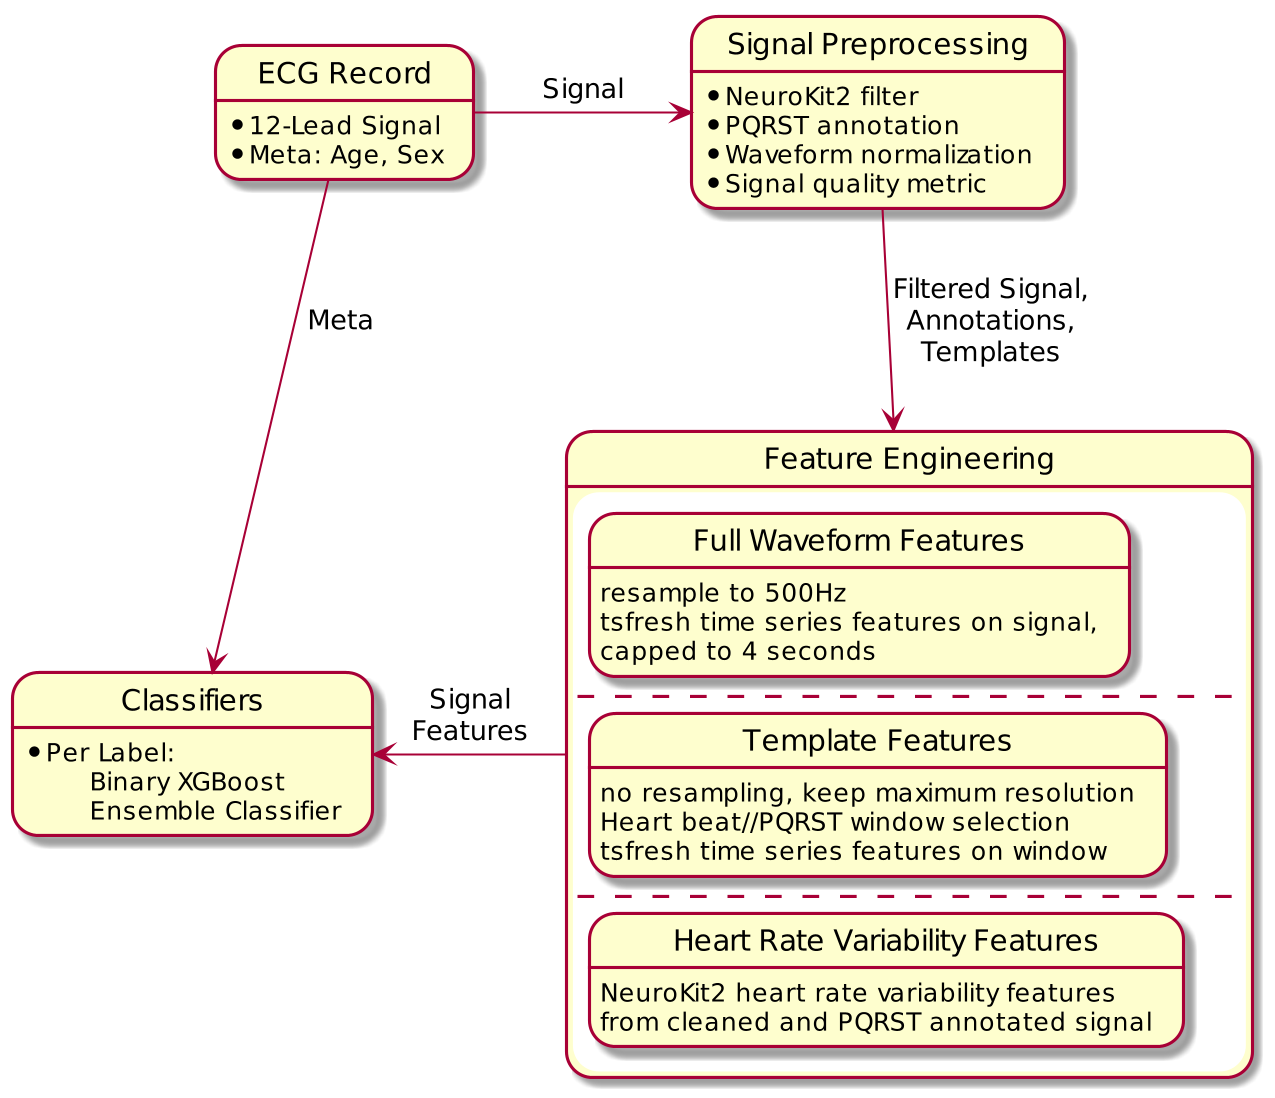
\includegraphics[width=7.9cm]{fig/methodology.png}
  \caption{Methodology overview. Feature engineering is performed concurrently for each lead then concatenated.}
  \label{fig:methodology}
\end{figure}

An overview our methodology is presented in Figure~\ref{fig:methodology}.

\subsection{Signal Pre-processing}

First, we filtered the raw signal using a finite impulse response filter, limited between 3 Hz and 45 Hz.
Next, we used the \emph{ecgpuwave} QRS detector to annotate each filtered signal lead, resulting in waveform start, end, and peaks for P-waves, T-waves, and R-waves~\cite{goldberger_ary_l_physiobank_2000}.
ECG PQRST templates were extracted by segmenting out continuous P-wave waveform starts to T-wave waveform ends.

For DTW template matching candidates, the extracted PQRST signals were first pooled by lead and label.
The BioSPPy implementation of the minimum distance template selection and clustering method was then used to isolate relevant templates per diagnosis~\cite{groupbiosppy_2015, uludag_biometric_2004}.

\subsection{Feature Engineering}

Our engineered features can be categorized as one of three categories: full waveform features, template features, and RR interval features.

\subsection{Classification}

We trained an XGBoost binary classifier to for each clinical diagnosis~\cite{chen_xgboost_2016}.


\section*{Acknowledgments}
We would like to thank Eric Ly and Leiah Luoma for their help and guidance during our research journey.

\bibliography{main}

\begin{correspondence}
Alexander W. Wong\\
Department of Computing Science\\
2-32 Athabasca Hall, University of Alberta\\
Edmonton, Alberta, Canada\\
T6G 2E8\\
alex.wong@ualberta.ca
\end{correspondence}

\end{document}

